\documentclass{article}
\usepackage[utf8]{inputenc}
\usepackage{fancyhdr}
\usepackage{lastpage}

\usepackage{float}

\usepackage{hyperref}
\usepackage{tikz} 
\usetikzlibrary{shapes,arrows}

\usepackage[margin=3cm]{geometry}
\usepackage{amssymb}
\usepackage{amsthm}
\usepackage{amsmath}
\usepackage{pgfgantt}
\graphicspath{{img/}{../img/}}


\usepackage{listings}
\lstset{
  basicstyle=\ttfamily,
  columns=fullflexible,
  frame=single,
  breaklines=true,
  postbreak=\mbox{\textcolor{red}{$\hookrightarrow$}\space},
}

\pagestyle{fancy}
\fancyhf{}
\begin{document}

\textbf{WHY WHY WHY?}

\section{Quadcopter Model}

For the physics model, the coordinate space is referred to using \emph{local tangent plane coordinates}, namely that $z$ is east, $x$ is north and $y$ is up. The principal axes of movement are \emph{pitch}, along the transverse ($z$) axis, \emph{roll}, along the longitudinal ($x$) axis, and \emph{yaw}, along the vertical ($y$) axis.

A UAV can be modelled as a rigid body with mass $m$, on Earth. As such, gravity acts on the agent at $9.81\frac{m}{s^2}$. The drag coefficient is estimated at $0.975$ considering the mass of the body \cite{Hattenberger}.

The dimensions and chracteristics of the agent have been determined using both realistic averages \cite{Figliozzi} and estimations. These can be seen in Fig. \ref{fig:dimensions}.

\begin{figure}[H]
    \centering
    \begin{tabular}{| c | c |} 
    \hline
    Parameter & Value \\ 
    \hline
    Mass, $m$ & 10 kg \\
    \hline
    Length, $l$ & 0.7 m \\
    \hline
    Width, $w$ & 0.7 m \\
    \hline
    Height, $h$ & 0.25 m \\
    \hline
    Propeller Area, $A$ & 0.16 m$^2$ \\
    \hline
    Distance To Propeller Centre, $d$ & 0.5 m \\
    \hline
    Drag Coefficient, $C_d$ & 0.975 \\
    \hline
    \end{tabular}
    \caption{Dimensions of the Agent}
    \label{fig:dimensions}
\end{figure}

The agent is modelled as a quadcopter, with four propellers. These can be independently controlled to affect the movement of the agent.

\begin{figure}[H]
    \centering
    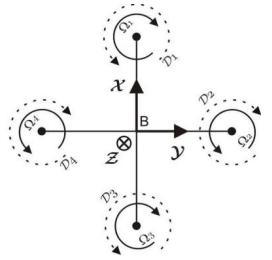
\includegraphics[height=80px]{prop.png}
    \hspace{1cm}
    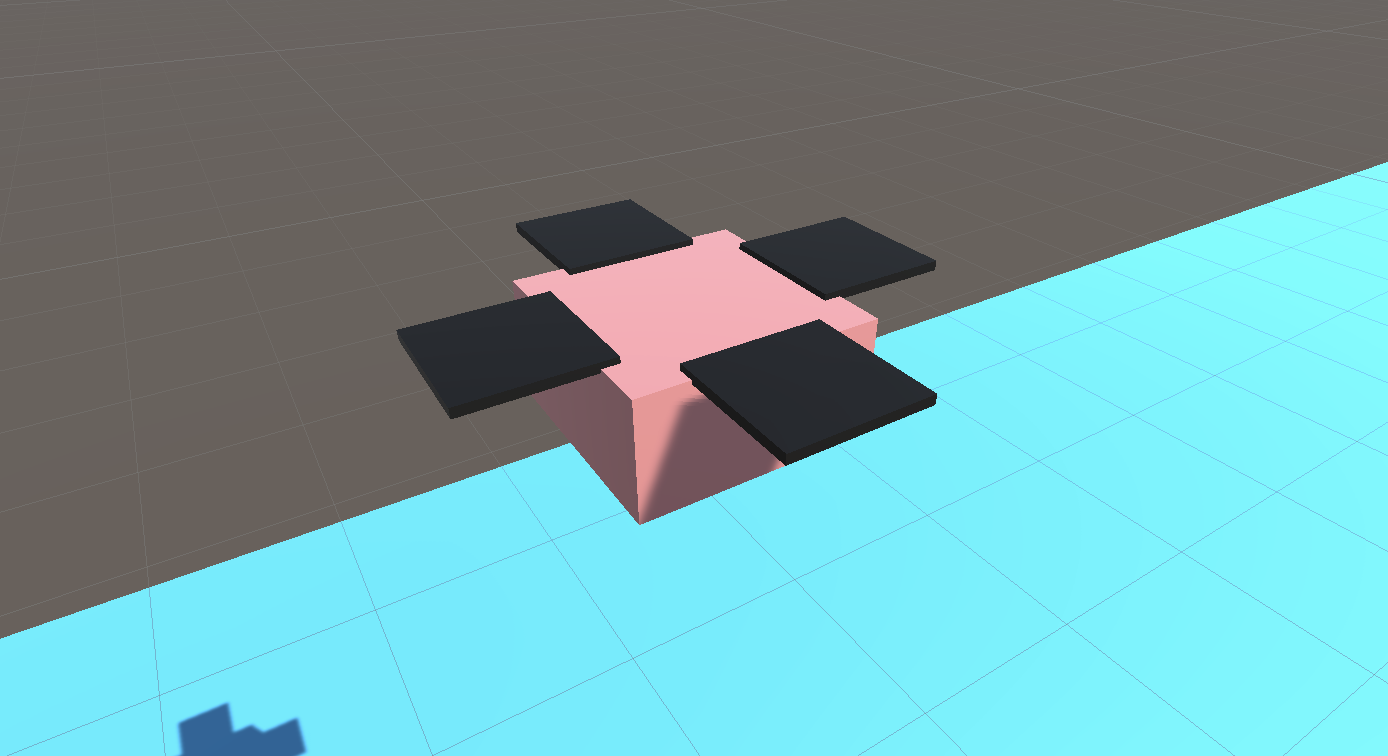
\includegraphics[height=80px]{drone-unity.png}
    \caption{Propeller Diagram \& Simulated Agent}
\end{figure}

For this investigation, a quadcopter was chosen as the type of agent, rather than a fixed-wing aircraft, due to increased maneouverability, simplicity when considering autonomous flight and simplicity in takeoff and landing procedures \cite{Thamm}.

There are four elements of control for an agent:
\begin{itemize}
    \item Roll angle (in radians), $\psi$
    \item Pitch angle (in radians), $\theta$
    \item Yaw rate (in $\frac{rad}{s}$), $\phi$
    \item Vertical thrust (in Newtons), $T$
\end{itemize}

For simplicity, these can be solely controlled by combinations of propeller thrust levels. 

A base thrust level, $T_b$, can be defined, which is the minimum thrust level required to maintain a stable hover. This is the thrust level required to counteract gravity, so $T_b = mg$. For each control operation, $T_b$ can be augmented by a thrust level, $T_{add}$, such that $|T_{add}| < T_b$, which is the additional thrust required to perform the operation.

As such, the control parameters can be operated by the following eight combinations of thrust levels for each propeller, with a high thrust level $T_{add} > 0$ and a low thrust level $T_{add} < 0$:


\begin{figure}[H]
    \begin{center}
    \begin{tabular}{| c | c | c |} 
    \hline
    Operation & High Thrust & Low Thrust \\ 
    \hline
    Positive Roll, $\psi_+$ & $D_4$ & $D_2$ \\
    \hline
    Negative Roll, $\psi_-$ & $D_2$ & $D_4$ \\
    \hline
    Positive Pitch, $\theta_+$ & $D_3$ & $D_1$ \\
    \hline
    Negative Pitch, $\theta_-$ & $D_1$ & $D_3$ \\
    \hline
    Positive Thrust, $T_+$ & $D_1, D_2, D_3, D_4$ & none \\
    \hline
    Negative Thrust, $T_-$ & none & $D_1, D_2, D_3, D_4$ \\
    \hline
    \end{tabular}
    \end{center}
    \caption{Control Operations and Thrust Levels}
    \label{fig:control}
\end{figure}


It is noted that yaw is omitted from Fig. \ref{fig:control}. For the purposes of the simulation, the propellers do not rotate. This lends itself to needing a workaround for simulating yaw. In \emph{Unity}'s physics engine, the rotation of opposite propellers can be simulated by applying forces along the $x$ and $z$ axes. As such, yaw is simulated according to the table below:

\begin{figure}[H]
    \begin{center}
    \begin{tabular}{| c | c | c |} 
    \hline
    Operation & Propeller & Direction of Force (respectively) \\ 
    \hline
    Positive Yaw, $\phi_+$ & $D_1, D_2$ & $Z_-, X_-$ \\
    \hline
    Positive Yaw, $\phi_+$ & $D_3, D_4$ & $Z_+, X_+$ \\
    \hline
    Negative Yaw, $\phi_-$ & $D_1, D_2$ & $Z_+, X_+$ \\
    \hline
    Negative Yaw, $\phi_-$ & $D_3, D_4$ & $Z_-, X_+$ \\
    \hline
    \end{tabular}
    \end{center}
    \caption{Yaw Directions and Respective Forces}
    \label{fig:yaw-control}
\end{figure}

In real world physics, a couple of propellers could not provide thrust in both extremes of the same axes, as they could not switch rotation direction. Likewise, forces in adjacent propellers would not cause rotation in the same direction. However, for the purposes of simplicity within the simulation, this is ignored.

It is then possible to set some thrust constants for each control operation. An example assigment for the pitch and roll operations is seen below in Fig. \ref{fig:thrust-constants}.

\begin{figure}[H]
    \begin{center}
    \begin{tabular}{| c | c | c |} 
    \hline
    Thrust Level & Thrust ($N$) \\ 
    \hline
    High & $\frac{2m \cdot g}{4}$\\
    \hline
    Normal & $\frac{m \cdot g}{4}$\\
    \hline
    Low & $\frac{0.5m \cdot g}{4}$\\
    \hline
    \end{tabular}
    \end{center}
    \caption{Thrust Constants for a drone of mass $m$ kg}
    \label{fig:thrust-constants}
\end{figure}

\section{Stabilisation: Proportional-Integral-Derivative Controller}

An issue arises with this implementation; the simulation becomes unstable as thrust cannot be provided in an accurate enough manner to counteract excessive rotation, notably in the roll and pitch axes. 

As such, the need for a control system becomes apparent. A PID (Proportional-Integral-Derivative) is a feedback control system, which uses the error between the current state and the desired state to calculate the control parameters.

Fig. \ref{fig:pid} shows the feedback loop of the PID controller. The error, $e(t)$, is calculated as the difference between the desired state, $r$, and the current state, $y$. The error is then fed into the three controllers. The output of each controller is then summed to produce the control variable, $u(t)$, which is then fed into the system. The system then produces the output, $y$, which is fed back into the error calculation.

\begin{figure}[H]
    \centering
    \tikzstyle{block} = [draw, fill=blue!20, rectangle, 
    minimum height=1em, minimum width=6em]
    \tikzstyle{sum} = [draw, fill=blue!20, circle, node distance=1cm]
    \tikzstyle{input} = [coordinate]
    \tikzstyle{output} = [coordinate]
    \tikzstyle{pinstyle} = [pin edge={to-,thin,black}]

    \begin{tikzpicture}[auto, node distance=2cm,>=latex']

    \node [input, name=input1] {};
    \node [sum, right of=input1] (sum) {$\Sigma$};
    \node [block, right of=sum, node distance=2.5cm] (I) {Integral};
    \node [block, above of=I, node distance=0.8cm] (P) {Proportional};
    \node [block, below of=I, node distance=0.8cm] (D) {Derivative};
    \node [sum, right of=I, node distance=2cm] (system) {$\Sigma$};
    \node [block, right of=system, node distance=2.5cm] (quad) {Quadcopter};
    \node [output, right of=quad] (output) {};

    \draw [draw,->] (input1) -- node {$r$} (sum);
    \draw [->] (sum) -- node {$e(t)$} (I);
    \draw [->] (sum) |- node {} (P.west);
    \draw [->] (sum) |- node {} (D.west);
    \draw [->] (I) -- node {} (system);
    \draw [->] (P) -| node {} (system);
    \draw [->] (D) -| node {} (system);
    \draw [->] (system) -- node {$u(t)$} (quad);
    \draw [->] (quad) -- node {$y$} (output);
    \draw [->] (quad.south) -- +(0,-1) -- +(-7.35,-1) -- node[] {-} (sum.200);
    \end{tikzpicture}
    \caption{PID Controller}
    \label{fig:pid}
\end{figure}


The PID controller is defined by three constant parameters, $K_p$, $K_i$ and $K_d$, which are the proportional, integral and derivative gains respectively. The control variable, $u(t)$, is then defined as:

$$u(t) = K_p e(t) + K_i \int_0^t e(\tau) d\tau + K_d \frac{de(t)}{dt}$$

where $e(t)$ is the error at time $t$. Considering our simulation operates in discrete time intervals (frames), this can be approximated, using the \emph{Laplace transform} as:

$$u(t) = K_p e(t) + K_i \frac{(e_t+e_{t-1})t}{2} + K_d \frac{e_t-e_{t-1}}{t}$$

Hence, a feedback loop of the entire system can be produced, taking into account different PID controllers for each control operation. This is shown in Fig. \ref{fig:pid-feedback}.

\begin{figure}[H]
    \centering
    \tikzstyle{block} = [draw, fill=blue!20, rectangle, 
    minimum height=1em, minimum width=6em]
    \tikzstyle{sum} = [draw, fill=blue!20, circle, node distance=1cm]
    \tikzstyle{input} = [coordinate]
    \tikzstyle{output} = [coordinate]
    \tikzstyle{pinstyle} = [pin edge={to-,thin,black}]

    \begin{tikzpicture}[auto, node distance=1.3cm,>=latex']

    \node [input, name=altitude] {$T$};
    \node [input, name=pitch, below of=altitude] {$\theta$};
    \node [input, name=roll, below of=pitch] {$\psi$};
    \node [input, name=yaw, below of=roll] {$\phi$};

    \node [block, right of=altitude, node distance=2.5cm] (alt) {$PID_{altitude}$};
    \node [block, right of=pitch, node distance=2.5cm] (pt) {$PID_{pitch}$};
    \node [block, right of=roll, node distance=2.5cm] (rl) {$PID_{roll}$};
    \node [block, right of=yaw, node distance=2.5cm] (yw) {$PID_{yaw}$};


    \node [input, name=guide1, right of=pt, node distance=2.5cm] {};
    \node [input, name=guide2, right of=rl, node distance=2.5cm] {};

    \node [block] (output) at ($(guide1)!0.5!(guide2)$) {Quadcopter};

    \draw [->] (altitude) -- node {$T$} (alt);
    \draw [->] (pitch) -- node {$\theta$} (pt);
    \draw [->] (roll) -- node {$\psi$} (rl);
    \draw [->] (yaw) -- node {$\phi$} (yw);

    \draw [->] (alt.east) -| +(0.2,+0.4) -- +(-2.5,+0.4) |- node[] {} (alt.170);
    \draw [->] (pt.east) -| +(0.2,+0.4) -- +(-2.5,+0.4) |- node[] {} (pt.170);
    \draw [->] (rl.east) -| +(0.2,+0.4) -- +(-2.5,+0.4) |- node[] {} (rl.170);
    \draw [->] (yw.east) -| +(0.2,+0.4) -- +(-2.5,+0.4) |- node[] {} (yw.170);

    \draw [->] (alt.east) -| node {} (output);
    \draw [->] (pt.east) -| node {} (output);
    \draw [->] (rl.east) -| node {} (output);
    \draw [->] (yw.east) -| node {} (output);

    \end{tikzpicture}
    \caption{System Model}
    \label{fig:pid-feedback}
\end{figure}

The constants are then tuned to generate expected stabilisation behaviour. As mentioned previously, each propeller has a base thrust level equal to the force required to hover, $T_b = \frac{mg}{4}$. The PID controller is then used to calculate the thrust level to be added to each propeller, $T_{add}$, in every frame of the simulation, to perform the desired operation.

Using manual tuning, the values were optimised as shown in Fig. \ref{fig:pid-tuning}

\begin{figure}[H]
    \centering
        \begin{tabular}{| c | c | c | c |} 
        \hline
        Control Operation & $K_p$ & $K_i$ & $K_d$ \\ 
        \hline
        Thrust & 6 & 5 & 2 \\
        \hline
        Pitch & 10 & 10 & 2 \\
        \hline
        Roll & 10 & 10 & 2 \\
        \hline
        Yaw & 10 & 10 & 2 \\
        \hline
        \end{tabular}
        \caption{Tuning Constants}
        \label{fig:pid-tuning}
\end{figure}

It is noted that the agent is slightly unstable at very small angles. This is negligible.

\section{Introducing Autonomy}
The initial aim is to achieve position control for an agent, such that when given a current position $[x_0,y_0,z_0]$ and a goal position $[x_1,y_1,z_1]$, the agent will move to the goal position.

There are several methods for this. An agent may yaw to face the goal, then pitch towards it. In the case of this project, time-sensitive position decisions will need to be made when considering swarm dynamics and collision avoidance, so a more efficient method is required. As such, the aim will be to pitch and roll towards the position.

This can be split up into two main goals:
\begin{enumerate}
    \item Apply a force in the opposite direction when avoiding other agents.
    \item Use trigonometry to apply relative $\phi$ and $\theta$ forces, reducing these forces when closer to the goal using a separate PID position controller.
\end{enumerate}

Initially, multiple agents are now introduced into the environment. They are programmed to hover. They should then move away from each other according to rule 1 above. This is the first principle that Reynolds \cite{Reynolds} introduced for autonomous agents - \emph{separation}.

\textbf{NB - note importance of both goals - should they be equal?}



\bibliographystyle{IEEEtran}
\bibliography{refs} 
\end{document}

